\chapter{Introduction}
\label{cha:introduction}

% general intro

Human languages obey many regularities which have been studied and formalized into laws.
One of the most well known such laws is Zipf's law, which states that
\begin{equation}
  \label{eq:zipf_law}
  p(i) \sim i^{-\alpha}
\end{equation}
where $i$ is a word's rank.
Generally, $\alpha \approx 1$. \cite{Zipf1949a}
This is the case not only for English but for every tested human language. \cite{Mehri2017}
Figure \ref{fig:zipf_languages_wiki} shows this relationship for the first 10 million words of Wikipedia dumps in 30 different languages.
This relationship also holds for artifical languages like Esperanto.
There have been many efforts to understand why this and other empiric laws occur consistently in human language.

\begin{figure}
  \centering
  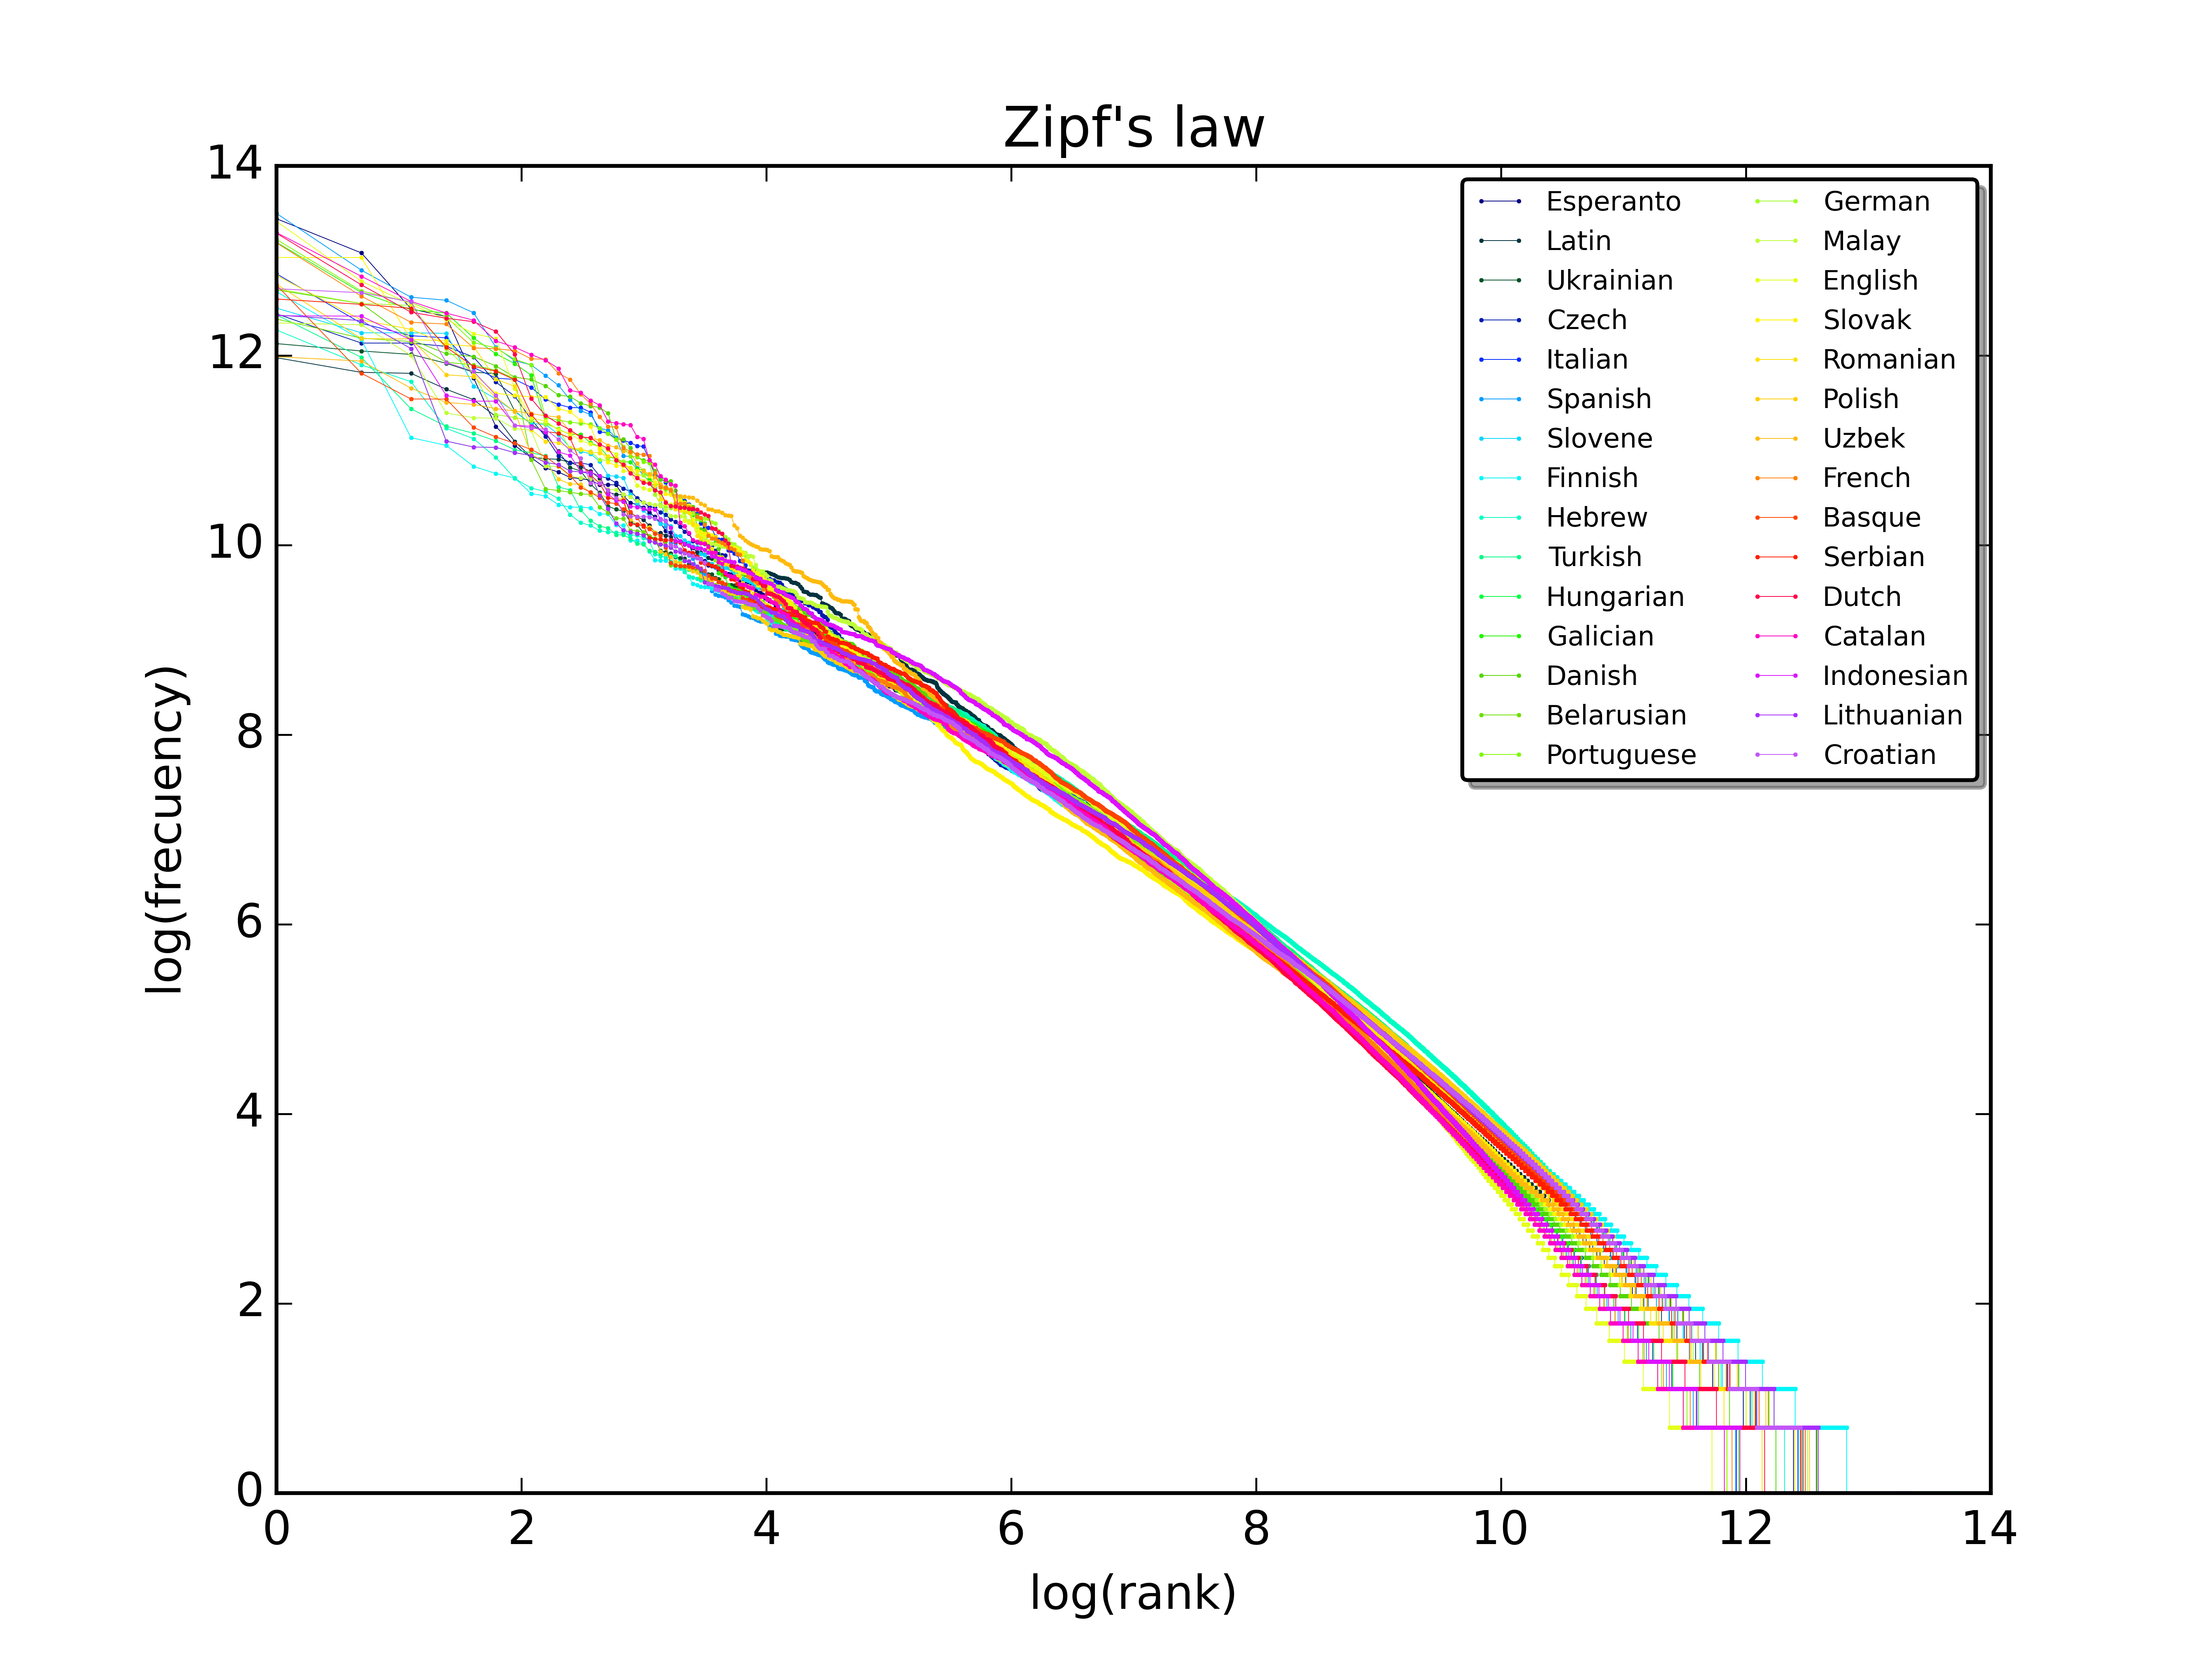
\includegraphics[width=\textwidth]{zipf_languages_wiki}
  \caption{
    The relationship of the logarithm of a word's frequency versus its rank for 30 human languages including Esperanto, an artifical language.
    Data from 30 Wikipedia dumps from October 2015.\\
    (Sergio Jimenez/Wikimedia, CC BY-SA 4.0 \cite{Jimenez2015a})}
  \label{fig:zipf_languages_wiki}
\end{figure}

% models and what their mean

This thesis focuses on a family of models \cite{Ferrer2007a} introduced initially to shed light into the origins of Zipf's law. \cite{Ferrer2005a} \cite{Ferrer2003a}
The family of models aims to explain language laws such as Zipf's law from the association of words and meanings.
The focus of this thesis are two models from this family, which were generalized with the addition of a new parameter $\phi$. \cite{Ferrer2018a}
They are referred to as the ``\firstmodel{}'' and the ``\secondmodel{}'' throughout.
The key difference between these two models is whether they consider meanings to follow a probability distribution \emph{internal} or \emph{external} to the model.
In the \firstmodel{} the probability of a meaning is determined entirely by the connections between words and meanings.
The \secondmodel{} determines the probability of a meaning in great part from an external \emph{a priori} probability distribution.
This \emph{a priori} probability can be considered the probability that the element referred to by the meaning is found in nature.
As an example, if elephants are rare but dogs are plentiful, the meaning ``elephant'' should be rarer than the meaning ``dog''.

% other language laws and models that explain them

In previous work \cite{Ferrer2003a} \cite{Ferrer2005a} Zipf's law of word frequencies has been predicted by the two models that are the focus of this thesis.
Just a few paragraphs ago this document opened with its formulation in Equation \eqref{eq:zipf_law}, the relationship between a word's frequency and frequency rank follows a power law.
But there exist other models that can explain language laws.
A popular explanation for Zipf's law of word frequencies is the random typing model.\cite{Miller1963a}
As a short summary, this model states that if characters are typed in sequence with a random chance of typing in a word separator then Zipf's law is reproduced.
There are a few issues with Miller's model, such as the assumption that words are independent from each other.
Random typing is often offered as a null hypothesis to the theory that Zipf's law comes from the \emph{principle of least effort} but even that has been called into question as it can also be considered a form of optimal coding. \cite{Ferrer2020a}

But Zipf's law for word frequencies is not the only linguistic law.
Zipf's meaning frequency law is not as popular as the word frequency law.
It states that the relationship between the number of meanings of a word, $\mu$, and its frequency, $f$, is \cite{Zipf1949a}
\begin{equation*}
  \mu \propto f^\delta.
\end{equation*}
Zipf derived the meaning-frequency law from his law of word-frequency, Equation \eqref{eq:zipf_law} and from his law of meaning distribution,
\begin{equation*}
  \mu \propto i^{-\gamma}
\end{equation*}
where $i$ is the rank of the word.

As with the constant $\alpha$, $\delta$ and $\gamma$ can be estimated using a regression method from data.

Zipf inferred $\delta \approx 1/2$ from $\gamma \approx 1/2$ and $\alpha = 1$.
Later on, others \cite{Ferrer2016a} have shown the relationship
\begin{equation}
  \label{eq:relation-exponents}
  \delta = \frac{\gamma}{\alpha}.
\end{equation}
between these exponents.

Miller's random typing model is not able to predict this other linguistic law as the meanings of the words are not taken into account.
It is also impossible for it to predict other more complex phenomena such as the vocabulary learning bias in children.
There are very good arguments \cite{Ferrer2018a} in favor of this family of models being able to predict this law and at least the \firstmodel{} has been able to predict vocabulary learning biases.
Both the case $\phi=0$ \cite{Ferrer2017a} and for the more generic formulation with any value of $\phi$ \cite{Carrera2021a}.

In his book \cite{Zipf1949a} Zipf argued also that older words (words that have existed in a language for a longer amount of time) would be more frequent.
This was tested empirically, as seen in Figure \ref{fig:zipf_word_ages}.

\begin{figure}
  \centering
  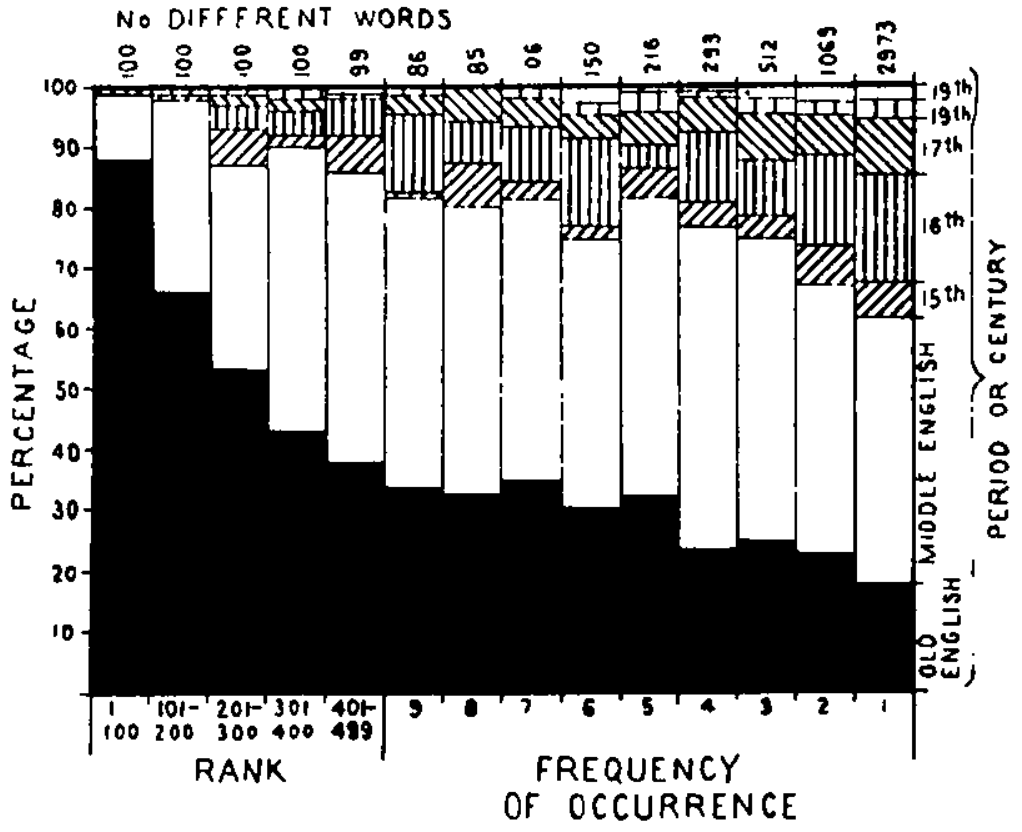
\includegraphics[width=\textwidth]{zipf_word_ages}
  \caption{
    Age of a word as a function of its frequency from Zipf's famous book. \cite{Zipf1949a}
    The right side of the $y$ axis indicates the historical period or century when a word was introduced and the left side the percentage of words.
    Each of the colors and patterns of the columns in the graph correspond with a time period.
    As indicated in the $x$ axis, the first five columns refer to the most common words by rank, while the next columns refer to the words with the specified frequency of occurrence.
  }
  \label{fig:zipf_word_ages}
\end{figure}

While this relationship between word frequencies and word ages could also not be predicted by random typing, there is another alternative model that can predict it.

Simon's model \cite{Simon1955} model argues that power laws appear as a result of the way the system is formed.
In the case of language, constant addition of new words and addition of new instances of already existing words at a rate proportional to the number of instances of a word
Here, time is a factor. And intuitively it seems that older words would indeed be more frequent.
However, Simon's model cannot explain the meaning distribution law as it does not take meaning into account and lacks the complexity to make predictions such as the vocabulary learning biases of children.

Table \ref{tab:comparison_models} shows a comparison between the two models seen here (random typing and Simon's model) and the two models that this thesis presents.
The two models are further fleshed out in following sections.

\begin{table}
  \centering
  \begin{adjustbox}{max width=\textwidth}
    \begin{threeparttable}
      \begin{tabular}{m{11.5em} C{4em} @{\hskip 1.5em} C{4em} @{\hskip 1.5em} C{4em} @{\hskip 1.5em} C{4em} @{\hskip 1.5em} C{4em} @{\hskip 1.5em} C{4em}}
        \toprule
        & Random Typing & Simon's Model & \Firstmodel{} ($\phi=0$) & \Secondmodel{} ($\phi=0$) & \Firstmodel{} ($\phi\neq 0$) & \Secondmodel{} ($\phi\neq 0$) \\
        \midrule
        \vspace{.75em} Rank-frequency law \vspace{.75em} & Yes \cellcolor{TableLightGreen} & Yes \cellcolor{TableLightGreen} & \cellcolor{TableLightGreen} Yes & \cellcolor{TableLightGreen} Yes & \cellcolor{TableLightRed} No & \cellcolor{TableLightGreen} Yes \\
        \addlinespace[.25em]
        \vspace{.75em} Meaning distribution law \vspace{.75em} & No \cellcolor{TableLightRed} & No \cellcolor{TableLightRed} & Yes \tnote{1} \cellcolor{TableLightYellow} & Yes \tnote{2} \cellcolor{TableLightGreen} & No \cellcolor{TableLightRed} & Yes \tnote{1} \cellcolor{TableLightYellow} \\
        \addlinespace[.25em]
        \vspace{.75em} Age-frequency law \vspace{.75em} & No \cellcolor{TableLightRed} & Yes \cellcolor{TableLightGreen} & Yes \cellcolor{TableLightGreen} & Yes \cellcolor{TableLightGreen} & Yes \cellcolor{TableLightGreen} & Yes \cellcolor{TableLightGreen} \\
        \addlinespace[.25em]
        \vspace{.75em} Vocabulary learning bias \vspace{.75em} & No \cellcolor{TableLightRed} & No \cellcolor{TableLightRed} & Yes \tnote{3} \cellcolor{TableLightGreen} & Unknown \cellcolor{TableLightBlue} & Yes \tnote{4} \cellcolor{TableLightGreen} & Unknown \cellcolor{TableLightBlue} \\
        \bottomrule
      \end{tabular}
      \begin{tablenotes}
        \item [1] Only based on the correlation sign.
        \item [2] See also \cite{Ferrer2016b} for mathematical reasoning.
        \item [3] As shown in previous work. \cite{Ferrer2017a}
        \item [4] As shown in an article \cite{Carrera2021a} derived from the work presented here.
      \end{tablenotes}
    \end{threeparttable}
  \end{adjustbox}
  \caption{
    A summary table comparing various models of human language.
    Columns show various models of human language: Random Typing and Simon's model.
    Then the two models studied in this thesis: \firstm{} and \secondmodel{}.
    The value of $\phi$ indicates whether it is the older version of the model (equivalent of the general model with $\phi=0$) or the more general version with $\phi \neq 0$.
    Rows show various predictions that these models could or could not do.
    The vocabulary learning bias was shown to be predicted with the \firstmodel{} and more recently with the more generic version of the model ($\phi \neq 0$)
  }
  \label{tab:comparison_models}
\end{table}

% models and optimization

Unlike Miller's and Simon's models, these models are based on the argument that human language is result of attempting to minimize the effort of both the speaker and the hearer. \cite{Ferrer2003a} \cite{Zipf1949a} Something that Zipf referred to as the \emph{principle of least effort}. That is why these models are based on the minimization of a cost function, which is calculated in terms of information theoretic measures.

This approach to optimization in human languages is not new.
Terry Regier argued \cite{Regier2007a} that color naming in human language corresponded with optimal partitions of the color space.
Regier's research showed that, indeed, color naming in many human languages was closely related to the optimal partitions of the color space.
The idea of language being ``optimal'' is not new.

From the computational point of view, an important aspect of the optimization process is the evaluation of the cost function.
The cost function can be evaluated \emph{statically}, recalculating it completely from scratch each time a change (or mutation) is made to the underlying graph.
However, it is possible to calculate only the changes that take place due to this mutation.
In this way the calculation is computationally less complex.
This is not a new approach, in shortest path calculation algorithms, when a change takes place it is common to adjust the result based on the change instead of recalculating the entire process. \cite{Buriol2003a}
The dynamic approach offers a significant speedup that justifies the issues that arise as a consequence, such as the increase in mathematical complexity and introduction of greater numerical error.

% the program exists ok

The tool developed to study these models is released under an open source license.
It is released with the hope that it will be useful to replicate these results, and also that it can be used to study similar models.

% outro

Now follows an introduction to the model.
It is not as in depth as what can be found in following chapters, but it does give the basic mathematical points of the models.

\section{Introduction to the model}
\label{sec:introduction_model}

This is a short introduction to the models presented in this thesis.
In this section, mathematical definitions and notation common to both models is given.
They will be used throughout the remainder of the thesis and specially throughout Chapter \ref{cha:methods} where a full explanation of both models is given.

Section \ref{sec:introduction_model_graph} presents the bipartite graphs that form the \emph{skeleton} of these models.
Section \ref{sec:introduction_model_info-theory} presents the information theoretic aspects, common to both models.
In Section \ref{sec:introduction_model_phi} the role of the $\phi$ parameter is explained.
Sections \ref{sec:introduction_model_first-model} and \ref{sec:introduction_model_second-model} cover the parts that unique to the \firstm{} and \secondmodel{} respectively. These are the \emph{flesh}, each covering the \emph{skeleton} in a different way.
Section \ref{sec:introduction_model_optimization} gives an overview of the optimization process.
Section \ref{sec:introduction_model_dynamic-static} explains the reasoning and difference of the static and dynamic versions of the implemented algorithms.

\subsection{Bipartite graph}
\label{sec:introduction_model_graph}

Both models studied in this thesis are based on the idea of a bipartite graph.
Bipartite graphs are comprised of two sets of elements and edges can only appear between an element of one set and an element of the other.

Our two sets are $S$ and $R$.
$S$ is a set of size $n$ containing all words.
The notation $s_i$ is used to refer to some element $i$ of the set $S$.
$R$ is a set of size $m$ containing all meanings.
The notation $r_j$ is used to refer to some element $j$ of the set $R$.

The bipartite graph is represented using the adjacency matrix $A_{n,m}$ (or simply $A$) in most cases.
$A_{n,m}$ is a \nbym{} binary matrix representing whether an edge exists or not in the graph.
Mathematically, each element of the matrix $A$ is defined as
\begin{equation*}
  %\label{eq:definition-aij}
  a_{i,j} =
  \begin{cases}
    1 & \text{if there exists an edge between $s_i \in S$ and $r_j \in R$} \\
    0 & \text{otherwise.}
  \end{cases}
\end{equation*}

In some cases it is more convenient to represent the bipartite graph as the set $E$ of all edges,
\begin{equation*}
  %\label{eq:definition-E}
  E = \Set{(s_i,r_j)}{\text{there exists an edge between $s_i \in S$ and $r_j \in R$}}.
\end{equation*}
For brevity, the pair $(s_i, r_j)$ is often represented as $(i,j)$.

The degree of the word $i$ is given as $\mu_i$, while the degree of a meaning $j$ is given as $\omega_j$.

Figure \ref{fig:graph-example-base} displays an example of a simple bipartite graph.
A graphical representation is included, as well as the corresponding values of the mathematical concepts discussed in this section up to here.

\begin{figure}
  \centering
  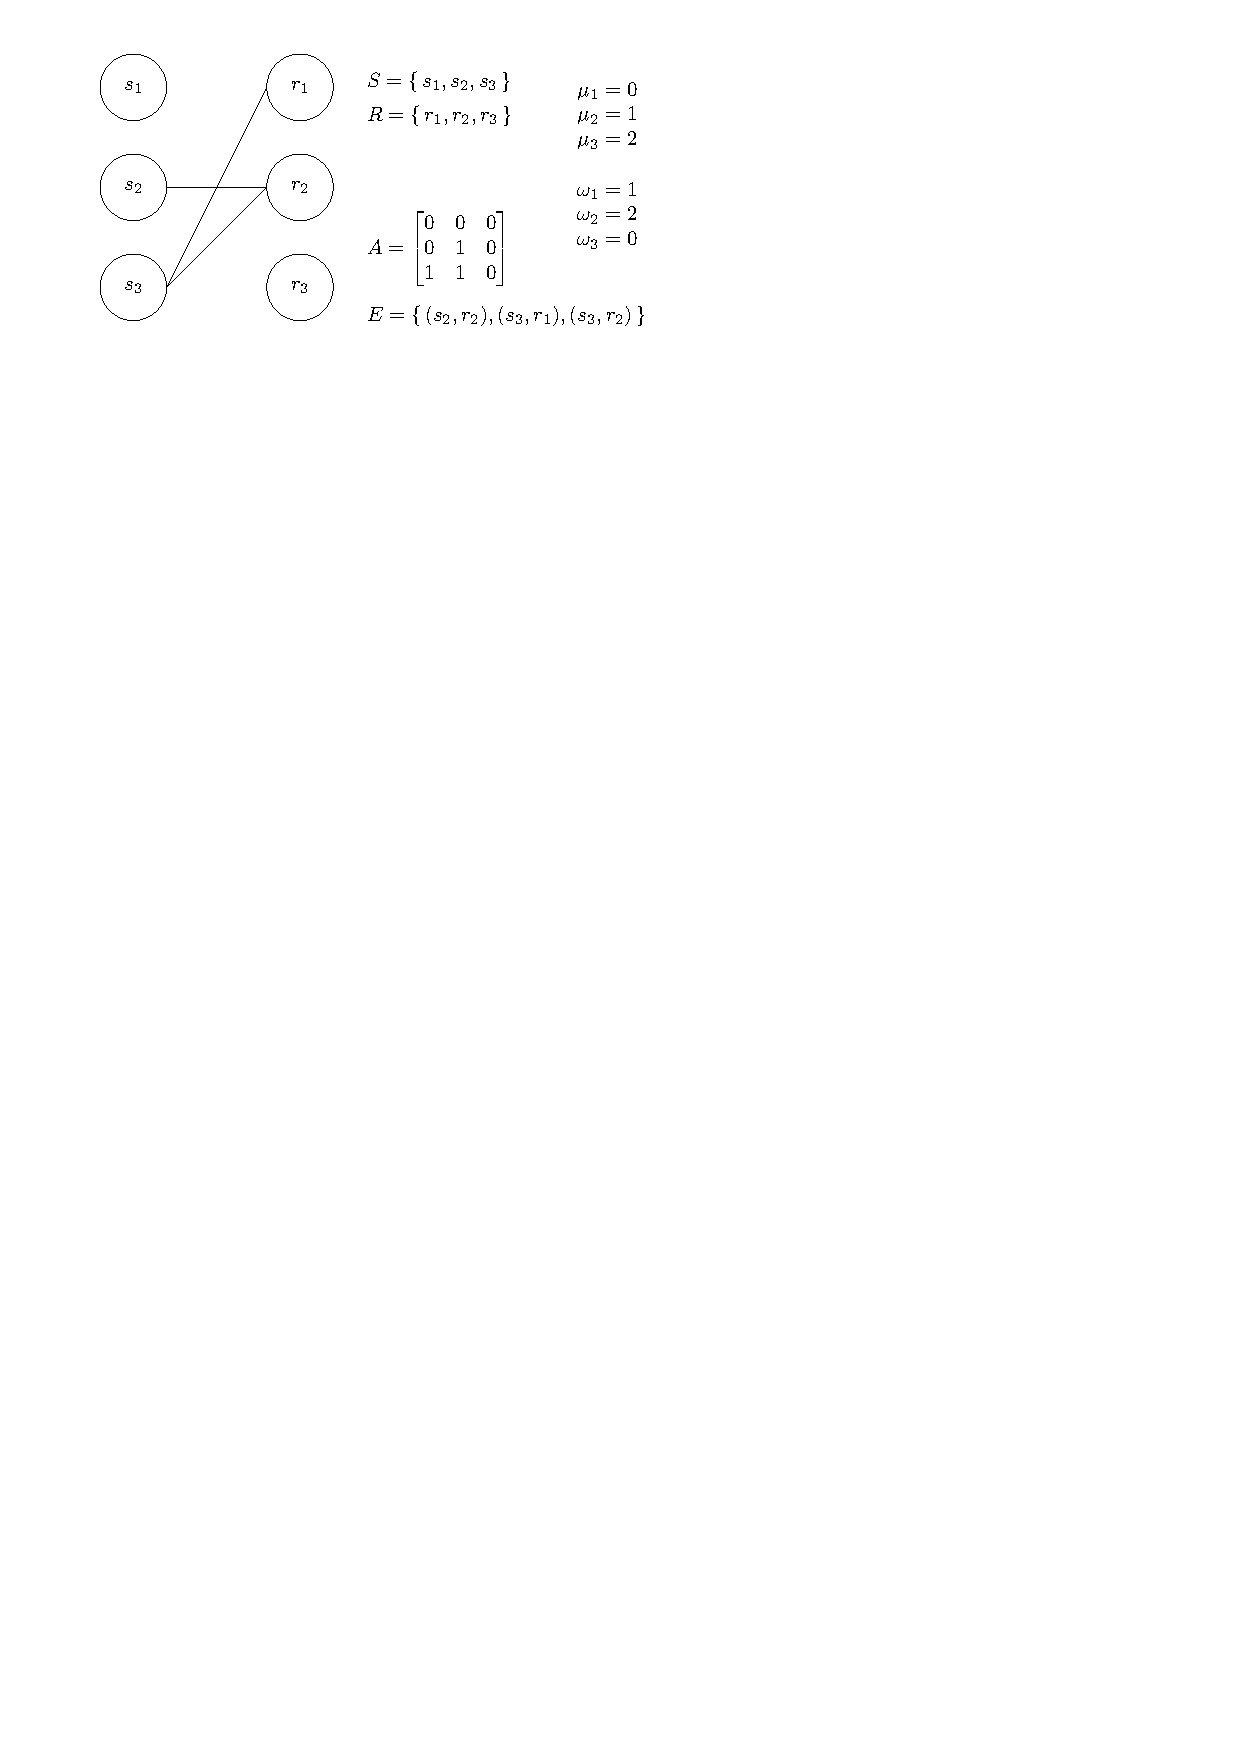
\includegraphics[width=\textwidth]{graph_example_base}
  \caption{%
    A bipartite graph with the corresponding adjacency matrix $A$, set of edges $E$ and vertex degrees $\mu$ and $\omega$ for each vertex.
  }
  \label{fig:graph-example-base}
\end{figure}

\subsection{Information theory}
\label{sec:introduction_model_info-theory}

Information theory measures are used to compute the cost function of the optimization process.
Here we go through a short overview of information theory formulas. They can be found in \cite{Cover1999}.

The general formula for the entropy of a set $X$ is
\begin{equation}
  \label{eq:definition-entropy-generic}
  H(X) = \sum_{x \in X} p(x) \log p(x)
\end{equation}
where $p(x)$ is the probability associated with the element $x$.
The general formula for the joint entropy of two sets $X$ and $Y$ is defined as
\begin{equation}
  \label{eq:definition-joint-entropy-generic}
  H(X,Y) = \sum_{x \in X} \sum_{y \in Y} p(x,y) \log p(x,y)
\end{equation}
where $p(x,y)$ is the joint probability of the elements $x$ and $y$.

Any other information theoretic measures concerning two sets can be obtained from $H(X)$, $H(Y)$ and $H(X,Y)$.
Mutual information
\begin{equation*}
  I(X,Y) = H(X) + H(Y) - H(X,Y),
\end{equation*}
and conditional entropies
\begin{equation*}
  H(X|Y) = H(X,Y) - H(X)
\end{equation*}
and
\begin{equation*}
  H(Y|X) = H(X,Y) - H(Y).
\end{equation*}
The diagram on Figure \ref{fig:relationships-entropies} shows these relationships in a more visual way.

\begin{figure}
  \centering
  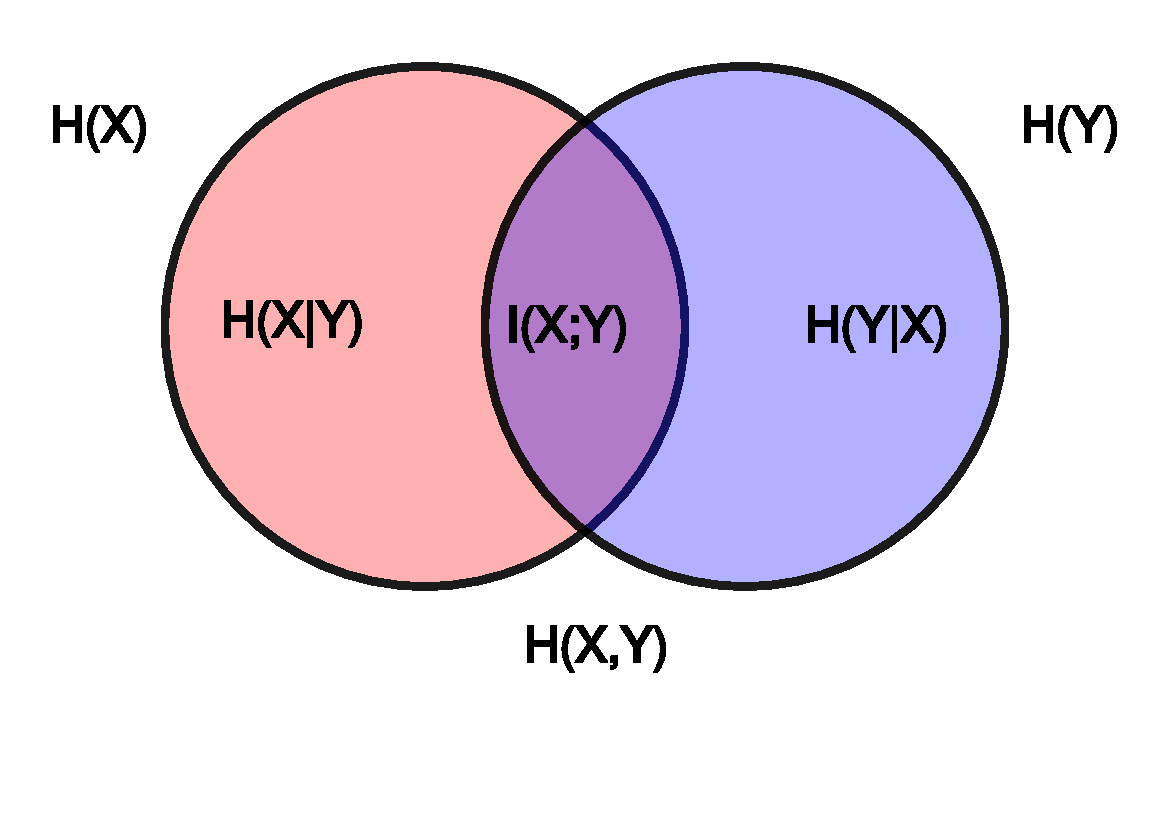
\includegraphics[width=\textwidth]{relationships_entropies}
  \caption{
    This diagram illustrates the relationships between information theoretic measures for two sets $X$ and $Y$.
    The area occupied by both left and right circle is the joint entropy $H(X,Y)$.
    The circle on the left (both the red and the violet areas) represents the marginal entropy $H(S)$ while the circle on the right (both blue and violet areas) represents the marginal entropy $H(Y)$.
    The red area is the conditional entropy $H(X|Y)$ while the blue area represents the conditional entropy $H(Y|X)$.
    The violet area represents the mutual information $I(X,Y)$.
  }
  \label{fig:relationships-entropies}
\end{figure}

Based on Equation \eqref{eq:definition-entropy-generic}, we define the entropies of words and meanings, $H(S)$ and $H(R)$ respectively, as
\begin{equation}
  \label{eq:definition-HS}
  H(S) = \sum_{i=1}^n p(s_i) \log p(s_i)
\end{equation}
and
\begin{equation}
  \label{eq:definition-HR}
  H(R) = \sum_{j=1}^m p(r_j) \log p(r_j).
\end{equation}
We also define the joint entropy of words and meanings, from Equation \eqref{eq:definition-joint-entropy-generic}, as
\begin{equation}
  \label{eq:definition-HSR}
  H(S,R) = \sum_{i=1}^n \sum_{j=1}^m p(s_i, r_j) \log p(s_i, r_j).
\end{equation}

\subsection{The $\phi$ parameter}
\label{sec:introduction_model_phi}

The $\phi$ parameter, which has already appeared up to this point, is used to generalize the older versions of the two main models studied.

In \cite{Ferrer2005a} and \cite{Ferrer2003a} these two models were introduced.
Later, the $\phi$ parameter is added to generalize the model and hopefully be able to predict more linguistic laws. \cite{Ferrer2018a}

As is presented in the following sections, when $\phi=0$, the older models are retrieved from the newer ones.

\subsection{The \firstmodel{}}
\label{sec:introduction_model_first-model}

In this model, the joint probability of a word $s_i$ and a meaning $r_j$ is proportional to the product of their degrees to the $\phi$ power.
When $\phi=0$, the joint probability depends only on whether there is a connection between the word and the meaning.
Mathematically,
\begin{equation*}
  \label{eq:psirj-proportional-mui-wj}
  p(s_i, r_j) \propto a_{i,j} (\mu_i \omega_j)^\phi.
\end{equation*}
When $\phi=0$ we recover a previous simpler model. \cite{Ferrer2005a}

The actual joint probability is derived from Equation \eqref{eq:psirj-proportional-mui-wj}, and from it the marginal probabilities of words and meanings are also derived.
Ultimately this leads to the information theoretic equations seen in Section \ref{sec:introduction_model_info-theory}.

\subsection{The \secondmodel{}}
\label{sec:introduction_model_second-model}

This model was introduced in \cite{Ferrer2003a} with meaning probabilities being constant and disconnected meanings being disallowed.
Here we present a generalization of the previous model.
In this model, the probability of a meaning $r_j$ is given \emph{a priori} as $\pi(r_j)$.
It is possible for a meaning to be disconnected from any words, in which case $p(r_j) = 0$.
In \cite{Ferrer2003a} disconnected meanings were disallowed and $\pi(r_j) = \frac{1}{m}$.
Additionally, $\phi=0$ in Equation \eqref{eq:prop-cond-prob_second-model}.
Here $\pi(r_j)$ can follow any probability distribution and disconnected meanings are allowed.
Zero values of $\pi(r_j)$ are disallowed, however, as meanings that could never occur are not the target of communication.

We then define $p(r_j)$ as
\begin{equation}
  \label{eq:prj-proportional-pirj}
  p(r_j) \propto (1 - \delta_{\omega_j,0}) \pi(r_j)
\end{equation}
where $\delta_{a,b}$ is the Kronecker delta,
\begin{equation*}
  \delta_{a,b} = \begin{cases}
    0 & \text{if}~a \neq b \\
    1 & \text{if}~a = b.
  \end{cases}
\end{equation*}
The word probability is then defined as the conditional probability of choosing a word given that a meaning has been chosen,
\begin{equation}
  \label{eq:prop-cond-prob_second-model}
  p(s_i | r_j) \propto a_{i,j} \mu_i^\phi.
\end{equation}

With the marginal meaning probability and the conditional probability of a word given a meaning, the joint probability and marginal word probability can be calculated.
From this the information theoretic equations are be obtained.

\subsection{Optimization}
\label{sec:introduction_model_optimization}

As seen in previous sections and will be seen in Section \ref{sec:introduction_hypothesis}, our hypothesis is that the empirical laws observed in human language are the result of minimizing the effort of speaker and hearer.

This effort is defined in terms of information theoretic measures.
We choose two competing forces.
$H(S)$, the entropy of the words, and $I(S,R)$, the mutual information between words and meanings.
It is the goal of any communications system to maximize $I(S,R)$. The smaller $I(S,R)$, the greater the effort for the hearer.
The higher the entropy of words, however, they harder they are to access.
When $H(S)=0$, only a single word has probability 1 while all others are 0, meaning that knowing which word to choose is trivial, while $H(S)$ is maximum when all words have equal probability, giving no indication of which should be chosen.

We define $\Omega(\lambda)$ as the cost function we aim to minimize,
\begin{equation}
  \label{eq:definition-Omega}
  \Omega(\lambda) = -\lambda I(S,R) + (1 - \lambda) H(S)
\end{equation}
where $0 \leq \lambda \leq 1$ is used to indicate the weight given to each of the two forces.
When $\lambda=0$, the minimization of $H(S)$ is completely favored while when $\lambda=1$ the maximization of $I(S,R)$ is.
When $\lambda=1/2$, they are equally favored.

The optimization process follows a Markov Chain Monte Carlo method at zero temperature.
It consists of making mutations to $A$, chancing $a_{i,j}$ from 1 to 0 or from 0 to 1.
If a set of mutations results in a decrease of $\Omega$, they are kept.
Otherwise they are undone and another set is attempted.

\subsection{Dynamic and static equations}
\label{sec:introduction_model_dynamic-static}

As is seen later on, in Chapter \ref{cha:model}, two sets of equations are derived for the information theoretic equations necessary to calculate $\Omega$ (Equation \eqref{eq:definition-Omega}).

A set of static equations recalculate everything from scratch.
The set of dynamic equations calculate the changes done only after a mutation to $A$ takes place.

As seen previously this dynamic recalculation can be more efficient.
In the case of this thesis, small changes are continuously done to the graph, making several mutations to $A$ then reevaluating $\Omega$.
Dynamically accounting for the differences brought about for these changes is much more efficient than recalculating every single measure each time.

Dynamic calculation, however, brings its own set of problems, such as the increase in mathematical complexity and the introduction of greater floating point error.
Section \ref{sec:introduction_goals} goes over this in more detail while Section \ref{sec:methods_model-implementation} covers the measures taken in order to deal with these problems.

Table \ref{tab:summary-computational} shows the computational costs of the two models for specific cases that are implemented in the \CC{} open source program.
The justification can be found in Section \ref{sec:model_compute}.

\begin{table}
  \centering
  \begin{adjustbox}{max width=\textwidth}
    \begin{tabular}{lcc}
      \toprule
                             & \Firstmodel{} & \Secondmodel{} \\
      \midrule
      Static                 & $\bigO{M}$                    & $\bigO{M}$                   \\
      Dynamic ($\phi\neq 0$) & $\bigO{\max(\mu_i,\omega_j)}$ & $\bigO{\max(\mu_i,|B_{i,j}|)}$ \\
      Dynamic ($\phi=0$)     & $\bigO{1}$                   & $\bigO{\mu_i}$                \\
      \bottomrule
    \end{tabular}
  \end{adjustbox}
    \caption{
      Summary table of the computational cost of each model and for particular cases.
      The columns indicate which of the two models and the rows the specific case for that model (static, dynamic general case for any value of $\phi$ and dynamic for the specific case of $\phi=0$ where simplifications are possible).
      The \firstmodel{} with $\phi=0$ originates from \cite{Ferrer2005a}.
      The \secondmodel{} with $\phi=0$ from \cite{Ferrer2003a}.
      The generalization where $\phi \neq 0$ for the family of models was introduced in \cite{Ferrer2018a} but without any simulation results.
      Each cell shows the computational complexity of updating the value of the cost function after mutating $a_{ij}$ (that is, the word $s_i$ and the meaning $r_j$ become connected from being disconnected or become disconnected from being connected).
      $M$ is the number of connections in the model.
      $\mu_i$ is the number of neighbors of the word ($s_i$) and $\omega_j$ the number of neighbors of the meaning ($r_j$).
      $|B_{i,j}|$ is the number of words that have at least one neighbor in common with $s_i$ including $r_j$.
    }
  \label{tab:summary-computational}
\end{table}

\section{Goals}
\label{sec:introduction_goals}

Here the goals of the thesis are explained.

Older models \cite{Ferrer2003a} \cite{Ferrer2005a} where $\phi=0$ can already make predictions.
Can these more generic models predict anything new? And can they still make the predictions  that the older models could?
These older less general models already predicted Zipf's word frequency law.
It would seem that the newer models should be able to make new predictions, such as the law of meaning frequency \cite{Ferrer2018a}.
And perhaps other laws, such as the age frequency law.
And of course, can they still predict the word frequency law?
So one of the goals is to investigate the linguistic laws predicted by the model, to see if the more general version can still make the same prediction as the previous models.
And also to investigate whether it can make new predictions about other linguistic laws.

The computational aspect of the model should also be taken into account.
The optimization process is key to the model, and it needs a stop condition.
However, it is not obvious to know what the right stop condition is.
The process might not reach a minimum due to not making enough attempts to continue minimizing the cost function before stopping.
And due to the size of the search space it is unfeasible to exhaustively search every possible neighboring state.
While the previous models with $\phi=0$ were analyzed mathematically \cite{Salge2015} \cite{Prokopenko2010}, when $\phi \neq 0$ they become more complex.
Another goal is to investigate whether the model reaches the local minimum.

Perhaps the main computational challenge is the recalculation of the cost function.
It must be as efficient as possible, but it must also be precise to not compromise the results.
To try to reduce the computational complexity of each step of the optimization process while keeping the results precise and relatively free of numerical error.
This implies not only the derivation of all the mathematics necessary to calculate the cost functions of the models, but also additional mathematical work to derive dynamic equations allowing for only a small part of the cost function to be recalculated.

However, dynamic equations introduce more numerical error from the fact that they imply subtracting ``old'' values and adding ``new'' ones.
Addition and subtraction operations can easily add numerical error to floating point operations.
If not dealt with, this error can accumulate and change the results.
An important goal, then, is to minimize numerical error originated by floating point operations without compromising efficiency.

Verification is also a very important point.
The mathematics of the model are complex, specially the dynamic version.
A single mistake can invalidate all the results obtained.
This is why the implementation must be tested thoroughly.

There is an engineering component.
The implementation and documentation of an open source tool allowing for the replication of the obtained results and also to further study these models.

This ties into another of the goals.
Science must be reproducible.
Previous work \cite{Ferrer2003a} \cite{Ferrer2005a} on this model suffered from a lack of reproducibility.
The results of this thesis should be completely open and easily reproducible.

\section{Hypothesis}
\label{sec:introduction_hypothesis}

Several hypothesis are stated here.

As seen in Chapter \ref{cha:introduction} and in \cite{Ferrer2018a}, there is a relationship between the exponents of the Zipf's word-frequency and meaning-frequency laws.
See Equation \eqref{eq:relation-exponents}.

The main hypothesis of the thesis is that linguistic laws appear due to an optimization process in the association of words and meanings.
In the model any effects of social interaction are neglected, which are the basis of other approaches to investigating human language such as the naming game. \cite{Baronchelli2006}

One of the questions that we seek to answer is whether local minima exist, as argued in \cite{Ferrer2017a}.

It is also hypothesized that when $\phi=1$ the models should be able to reproduce Zipf's meaning-frequency law, as seen in \cite{Ferrer2018a}.

\redtxt{It is hypothesized that the initial condition of the optimization process plays an important role in determining the outcome of the optimization process.
We use several configurations that are known to be maximums or minimums of the cost function in order to explore the effect that the initial condition of the graph has in the final outcomes.}

\section{Outline of the thesis}
\label{sec:introduction_outline}

The rest of the thesis is organized as follows:

In Chapter \ref{cha:model} the mathematical and computational aspects of the models are covered in detail.
From the basic assumptions outlined in Section \ref{sec:introduction_model} the formulas for marginal and joint probabilities of words and meanings are derived and, from them, the information theoretic measures needed to compute the cost function.
The dynamic equations are then derived from the static ones. The extreme cases (when there is only one connection between a word and a meaning or when every word is connected to every meaning, etc) are given as well as the invariants, the maximum and minimum possible values that the information theoretic measures can achieve.
These steps are repeated for both the \firstm{} and \secondmodel{}.
Along the way several properties are given, which are elaborated on in the Appendix along with some derivations that might be excessively long.
For the computational aspect, the computational complexity of the static and dynamic versions of the computation of the cost function are shown.
For the dynamic version a distinction is made between the general case and the case when $\phi=0$.
Again, the complexity is shown for both the \firstm{} and \secondmodel{}.
Table \ref{tab:summary-computational} summarizes the complexity for the various methods of calculating the cost function in both models.

Chapter \ref{cha:methods} goes into the more tangible details of the implementation of the model beyond just mathematics: the implementation decisions and various algorithms, a diagram of the class hierarchy of the implementation (Figure \ref{fig:class-diagram}), the algorithms for the generation of the initial random graphs, the strategies used to deal with numerical error from floating point arithmetic are all outlined and the methods used to obtain several probability distributions for $\phi$ are all shown.
The optimization algorithm is covered in more detail including the choices for a stop condition.
The choices regarding parallelization of the algorithms and why it was decided to not make the algorithms parallel.
Details about the verification of the model are given, including all the strategies used to ensure that the dynamic and static implementations were equivalent.
The chapter closes with the problems encountered and how they were dealt with, both the numerical precision problems and the rest of problems encountered.

Chapter \ref{cha:results} presents the results obtained.
Results from previously published papers \cite{Ferrer2005a} \cite{Ferrer2003a} are replicated.
This both deals with the reproducibility issues in those works and serves as a benchmark to verify that the model is consistent with previous results.
New data obtained for $\phi=1$ and both models is presented.
This data includes the evolution of the values of the information theoretic measures of the optimal graphs for values of $\lambda$ ranging from 0 to 1.
Certain statistical measures are shown for select values of $\lambda$, including several of the relationships between frequency, frequency rank, degree (number of meanings of a word) and degree rank.
Values of the exponents and factors of the observed power laws are obtained with a Theil-Sen estimator.

Chapter \ref{cha:discussion} discusses the results obtained and introduces some possible future work.
Quantitative linguistics subjects are discussed, previously introduced word laws are compared with the data and it is argued whether the presented models can reproduce them and to what degree.
These laws include the word frequency law, the meaning frequency and meaning distribution laws and the age frequency law.
The computational results are also discussed, specifically regarding local minima of the cost function.
The section closes with a review of future work.
Alternative optimization methods are commented on, simulated annealing and gradient descent.
Other possible predictions of the \secondmodel{}, such as the vocabulary learning already studied for the \firstmodel{} \cite{Ferrer2017a} \cite{Carrera2021a}.
Possible further improvements to the numerical error problems are also commented.

%%% Local Variables:
%%% mode: latex
%%% TeX-master: "tfm"
%%% End:
